\section{PS12, Ex. 1 (A): Job-market signaling}

\begin{frame}{PS12, Ex. 1 (A): Job-market signaling}
    \begin{multicols}{2}
      \textit{(A)} Consider figure 4.2.8 in Gibbons\\
      (p. 201). Remind yourselves about the separating equilibrium related to the figure. Why can the high type not choose $e^*(H)$ in a separating equilibrium?\vspace{8pt}
      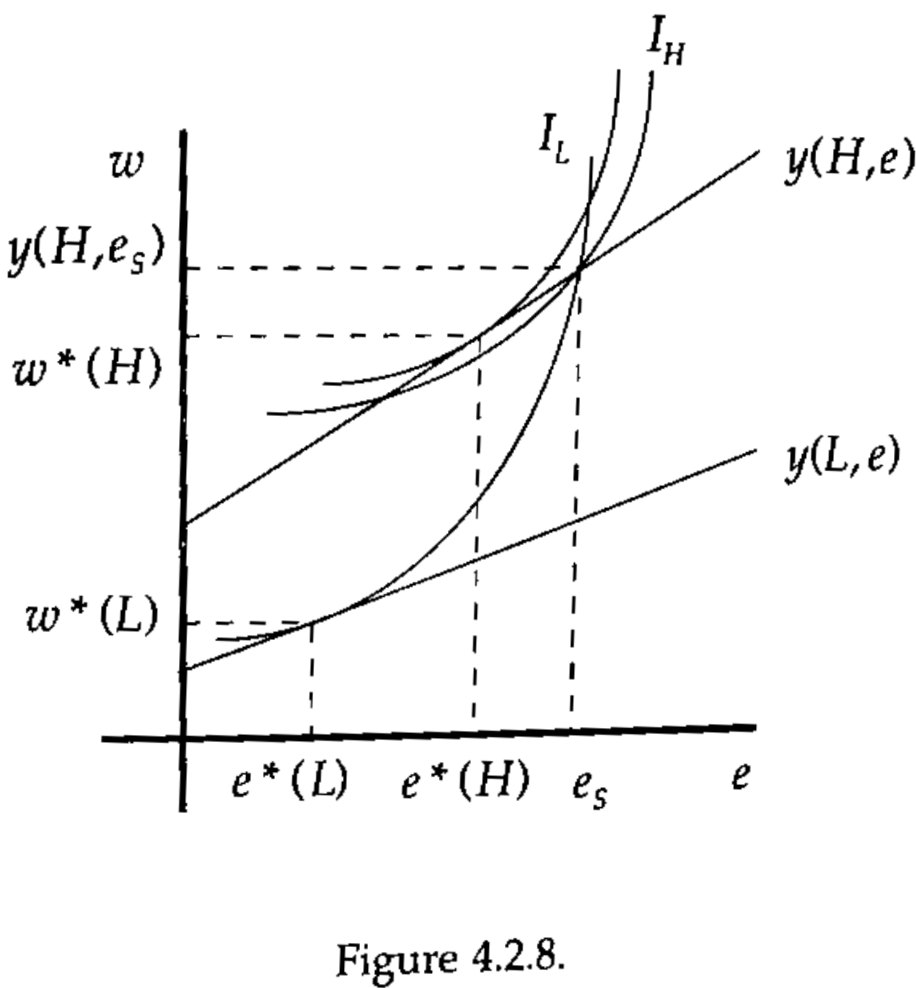
\includegraphics[width=\columnwidth]{figures/Gibbons428}
      \vfill\null\columnbreak
      \begin{itemize}
        \item[Step 1:] \textbf{Explain the graphs $\bm{I_L,I_H,y(L,e),y(H,e)}$.}
      \end{itemize}
      \vfill\null
    \end{multicols}
\end{frame}
\begin{frame}{PS12, Ex. 1 (A): Job-market signaling}
    \begin{multicols}{2}
      \textit{(A)} Consider figure 4.2.8 in Gibbons\\
      (p. 201). Remind yourselves about the separating equilibrium related to the figure. Why can the high type not choose $e^*(H)$ in a separating equilibrium?\vspace{8pt}
      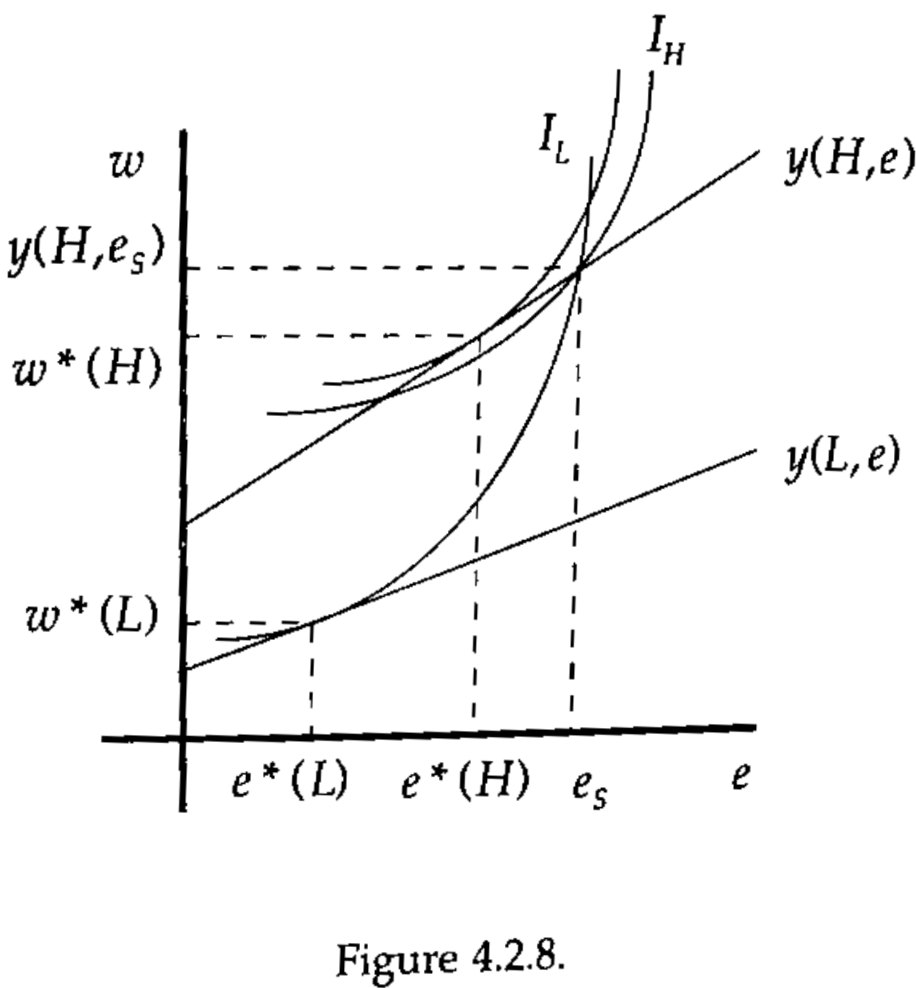
\includegraphics[width=\columnwidth]{figures/Gibbons428}
      \vfill\null\columnbreak
      \begin{itemize}
        \item[Step 1:] Explain $I_L,I_H,y(L,e),y(H,e)$:
      \end{itemize}\vspace{-6pt}
      For each type of worker $\eta\in L,H$:\vspace{-6pt}
      \begin{itemize}
        \item[$I_\eta$:] The indifference curve over which the worker's utility is constant.
        I.e. how much the wage must increase to compensate for higher education.
        \item[$y(\eta,e)$:] \vspace{-2pt} The expected output of a worker with ability $\eta$ and education $e$ which is equal to the wage offered by the firms under competition.\\
        I.e. education is now productive and more so for the high-ability worker.
      \end{itemize}\vspace{-6pt}
      Under complete information, the optimal education is where a worker's indifference curve is tangent to her productivity.\vspace{-6pt}
      \begin{itemize}
        \item[Step 2:] \textbf{Why can \textit{H} not choose $\bm{e^*(H)}$ in a separating equilibrium?}
      \end{itemize}
      \vfill\null
    \end{multicols}
\end{frame}
\begin{frame}{PS12, Ex. 1 (A): Job-market signaling}
    \begin{multicols}{2}
      \textit{(A)} Consider figure 4.2.8 in Gibbons\\
      (p. 201). Remind yourselves about the separating equilibrium related to the figure. Why can the high type not choose $e^*(H)$ in a separating equilibrium?\vspace{8pt}
      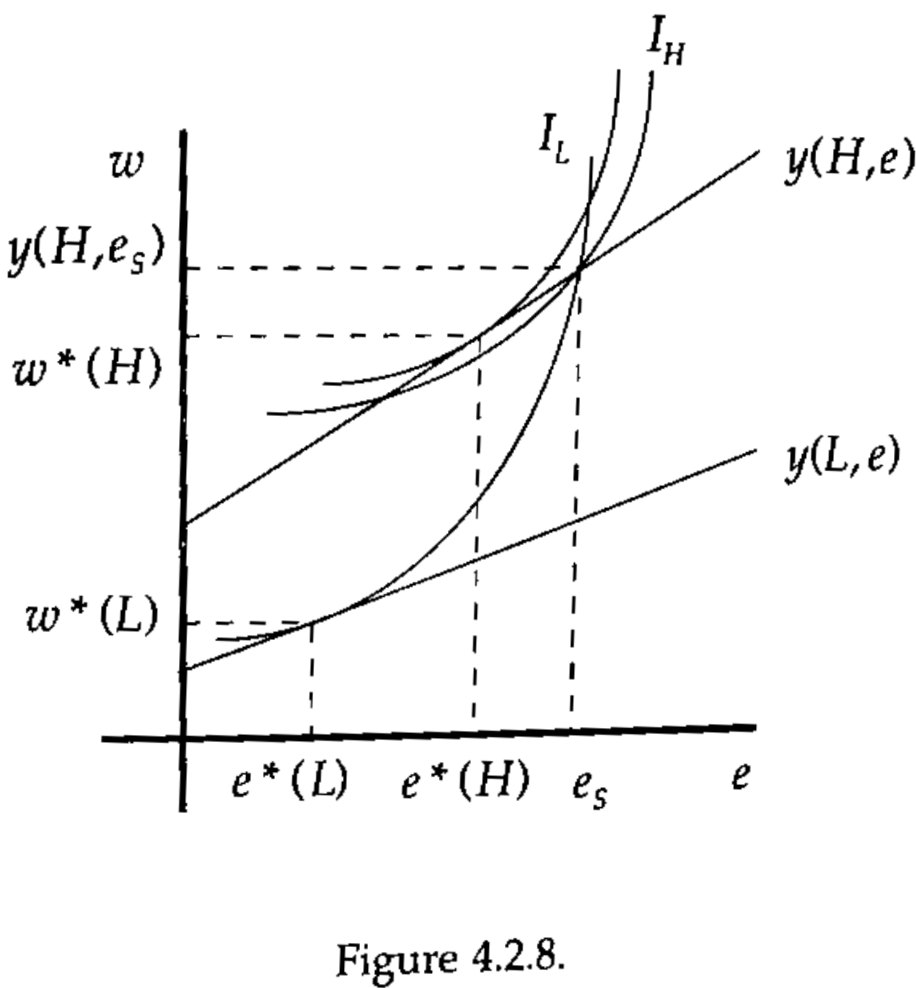
\includegraphics[width=\columnwidth]{figures/Gibbons428}
      \vfill\null\columnbreak
      \begin{itemize}
        \item[Step 1:] Explain $I_L,I_H,y(L,e),y(H,e)$:
      \end{itemize}\vspace{-8pt}
      For each type of worker $\eta\in L,H$:\vspace{-8pt}
      \begin{itemize}
        \item[$I_\eta$:] The indifference curve over which the worker's utility is constant.
        I.e. how much the wage must increase to compensate for higher education.
        \item[$y(\eta,e)$:] \vspace{-4pt} The expected output of a worker with ability $\eta$ and education $e$ which is equal to the wage offered by the firms under competition.\\
        I.e. education is now productive and more so for the high-ability worker.
      \end{itemize}\vspace{-8pt}
      Under complete information, the optimal education is where a worker's indifference curve is tangent to her productivity.\vspace{-8pt}
      \begin{itemize}
        \item[Step 2:] Why can $H$ not choose $e^*(H)$?
      \end{itemize}\vspace{-6pt}
      In a separating equilibrium, the firms perfectly identify $H$ and $L$ by education choices. However, as $[e^*(H),w^*(H)]$ is above $L$'s indifference curve, $L$ would imitate $H$. Thus, $H$ needs to increase education to $e_s$ to credibly signal type $H$.% though this lowers her utility.
      \vfill\null
    \end{multicols}
\end{frame}
